%----------------------------------------------------------------------------------------
%	PACKAGES AND THEMES
%----------------------------------------------------------------------------------------
\documentclass[aspectratio=169,xcolor=dvipsnames]{beamer}
\usetheme{Simple}

\usepackage{hyperref}
\usepackage{graphicx} % Allows including images
\usepackage{booktabs} % Allows the use of \toprule, \midrule and \bottomrule in tables
\usepackage{amsmath}
\usepackage{multimedia}

%----------------------------------------------------------------------------------------
%	TITLE PAGE
%----------------------------------------------------------------------------------------

% The title
\title[short title]{Numeric simulation using finite elements}
\subtitle{Sparse but not scarce}

\author {Martin Fasser, Charlotte Vavourakis}
\institute[UIBK] % Your institution may be shorthand to save space
{
    % Your institution for the title page
    University of Innsbruck
    \vskip 3pt
}
\date{\today} % Date, can be changed to a custom date


%----------------------------------------------------------------------------------------
%	PRESENTATION SLIDES
%----------------------------------------------------------------------------------------

\begin{document}

\begin{frame}
    % Print the title page as the first slide
    \titlepage
\end{frame}

%\begin{frame}{Overview}
    % Throughout your presentation, if you choose to use \section{} and \subsection{} commands, these will automatically be printed on this slide as an overview of your presentation
%    \tableofcontents
%\end{frame}

%------------------------------------------------
%\section{First Section}
%------------------------------------------------

%------------------------------------------------
%\section{Second Section}
%------------------------------------------------

\begin{frame}{Original implementation: dense matrix}
%    Show recording (or t0/tend) of the solution
    \begin{center}
    \movie{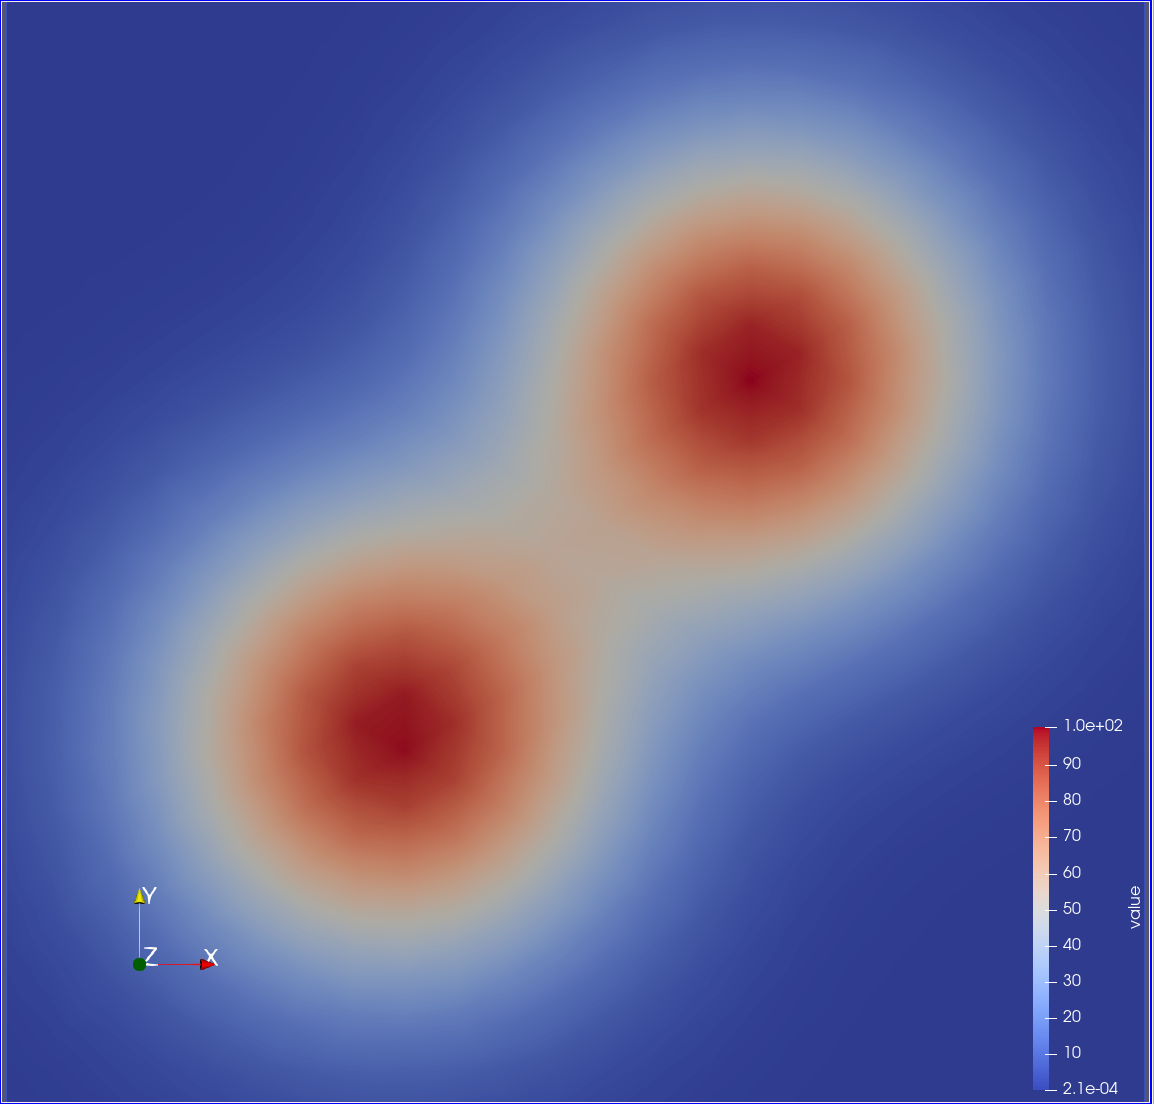
\includegraphics[width=0.5\textwidth]{thumbnail.png}}{two_blobs.avi}
    \end{center}
\end{frame}

%------------------------------------------------
\begin{frame}{Why Sparse?}
    \begin{columns}[c] % The "c" option specifies centered vertical alignment while the "t" option is used for top vertical alignment

        \column{.45\textwidth} % Left column and width
        
        \textbf{Storage space}
        \begin{center}
    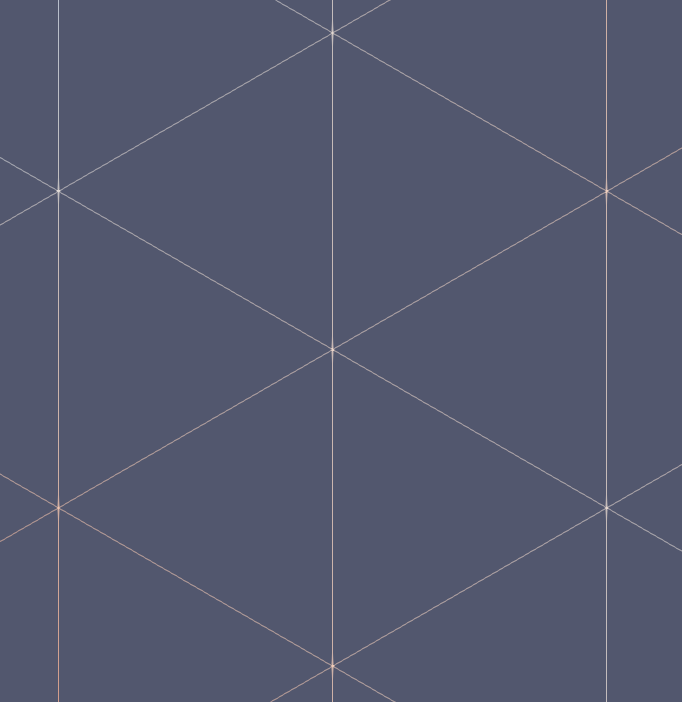
\includegraphics[width=0.3\linewidth]{mesh.png}
    \end{center}
        \begin{enumerate}
        	\item $N=$ number of mesh points
            \item $\approx \; 6 \cdot N $ -nonzero elements in matrix
            \item storage for dense matrix ($\propto N^2$): \\ 2.11 MB
            \item storage for sparse matrix ($\propto N$): \\ 0.05 MB
        \end{enumerate}

        \column{.5\textwidth} % Right column and width
        \begin{center}
    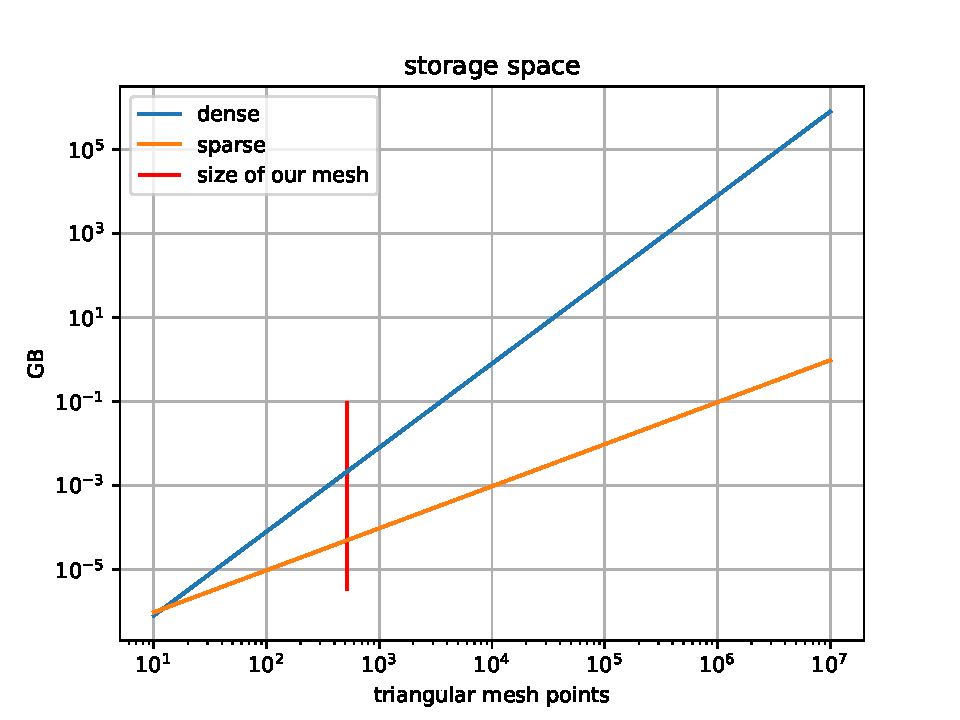
\includegraphics[width=1\linewidth]{storage_space.pdf}
    \end{center}

    \end{columns}
\end{frame}

%------------------------------------------------

\begin{frame}{Assignment: Sparse but not scarce}
	\begin{itemize}
	    \item Convert PDE solver matrix to sparse format and compare the performance with your
	dense matrix implementation.
		\item Use library implementation and compare it with a self-implemented CSR format.

	\end{itemize}
\end{frame}

%------------------------------------------------
\begin{frame}{Different Sparse Formats}
    \begin{columns}[c] % The "c" option specifies centered vertical alignment while the "t" option is used for top vertical alignment

\column{.65\textwidth} % Left column and width
\begin{itemize}
\item sparse - manual
  \begin{itemize}
     	\item $\mathrm{values} =  \begin{bmatrix} 
		5.3, & 1.5, & 4.2, & 3.1, & 2, & 2.2, & 1.9 
		\end{bmatrix}$

		\item $\mathrm{pos} = \begin{bmatrix}
		1, & 4, & 5, & 7, & 9, & 18, & 20 
		\end{bmatrix}$
	\end{itemize}
\item sparse - coo (coordinate list)
	\begin{itemize}
		\item $\mathrm{values} = \begin{bmatrix}
		5.3, & 1.5, & 4.2, & 3.1, & 2, & 2.2, & 1.9 
		\end{bmatrix}$
		\item $\mathrm{col\_ind} = \begin{bmatrix}
		1, & 4, & 0, & 2, & 4, & 3, & 0 
		\end{bmatrix}$
		\item $\mathrm{row\_ind} = \begin{bmatrix}
		0, & 0, & 1, & 1, & 1, & 3, & 4 
		\end{bmatrix}$
	\end{itemize}
\item sparse - csr (compressed row storage)
	\begin{itemize}
       \item $\mathrm{values} = \begin{bmatrix}
		5.3, & 1.5, & 4.2, & 3.1, & 2, & 2.2, & 1.9 
		\end{bmatrix}$
		\item $\mathrm{col\_ind} = \begin{bmatrix}
		1, & 4, & 0, & 2, & 4, & 3, & 0 
		\end{bmatrix}$
		\item $\mathrm{row\_ptr} = \begin{bmatrix}
		0, & 2, & 5, & 5, & 6, & 7 
		\end{bmatrix}$
	\end{itemize}
\end{itemize}
        
        \column{.3\textwidth} % Right column and width
        $ \left( \begin{array}{rrrrr} 
0 & 5.3 & 0 & 0 & 1.5\\ 
4.2 & 0& 3.1 & 0 & 2\\ 
0 & 0 & 0 & 0 & 0 \\
0 & 0 & 0 & 2.2 & 0 \\
1.9 & 0 & 0 & 0 & 0
\end{array} \right) $

    \end{columns}
\end{frame}

%------------------------------------------------
\begin{frame}{Matrix assembly}

\begin{columns}[c]

\column{.4\textwidth} % Left column and width

class $\mathrm{sparse\_mat}$:

\begin{center}
    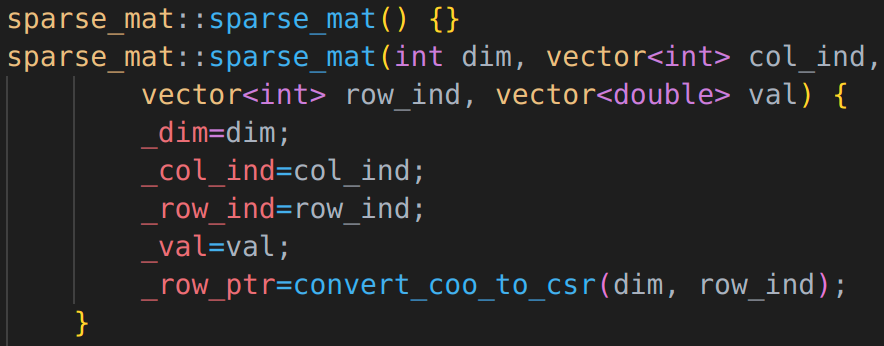
\includegraphics[width=0.9\linewidth]{class_sparsematrix.png}
    \end{center}


        
\column{.55\textwidth} % Right column and width
       preliminaries: \\
\begin{center}
    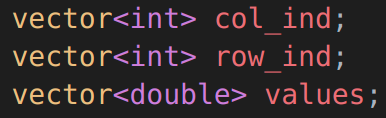
\includegraphics[width=0.4\linewidth]{sparse_construct.png}
    \end{center}

filling:
 
\begin{center}
    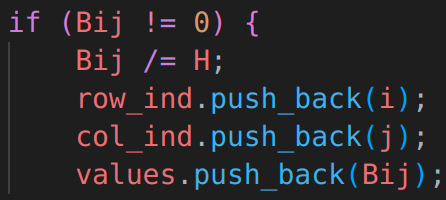
\includegraphics[width=0.5\linewidth]{sparse_fill.png}
    \end{center}

constructing the $\mathrm{sparse\_mat}$ object: \\
\begin{center}
    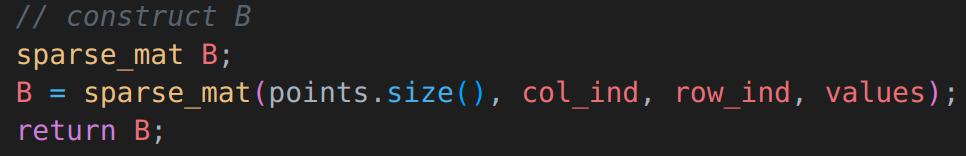
\includegraphics[width=0.9\linewidth]{sparse_create.png}
    \end{center}
    \end{columns}


\end{frame}

%------------------------------------------------
\begin{frame}{Matrix assembly: Conversion coo to csr}
    \begin{columns}[c] % The "c" option specifies centered vertical alignment while the "t" option is used for top vertical alignment

\column{.65\textwidth} % Left column and width
coo format: \\
$\mathrm{row\_ind} = \begin{bmatrix}
		0, & 0, & 1, & 1, & 1, & 3, & 4 
		\end{bmatrix}$

\begin{center}
    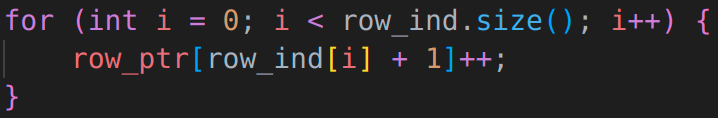
\includegraphics[width=0.7\linewidth]{conversion1.png}
    \end{center}

how many elements in each row:
$\mathrm{row\_step} = \begin{bmatrix}
		0, & 2, & 3, & 0, & 1, & 1 
		\end{bmatrix}$

\begin{center}
    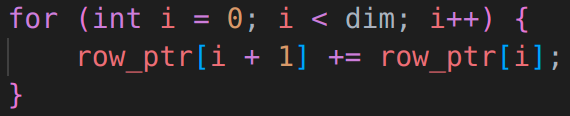
\includegraphics[width=0.7\linewidth]{conversion2.png}
    \end{center}

csr format: \\
$\mathrm{row\_ptr} = \begin{bmatrix}
		0, & 2, & 5, & 5, & 6, & 7 
		\end{bmatrix}$

        
\column{.3\textwidth} % Right column and width
        $ \left( \begin{array}{rrrrr} 
0 & 5.3 & 0 & 0 & 1.5\\ 
4.2 & 0& 3.1 & 0 & 2\\ 
0 & 0 & 0 & 0 & 0 \\
0 & 0 & 0 & 2.2 & 0 \\
1.9 & 0 & 0 & 0 & 0
\end{array} \right) $

    \end{columns}
\end{frame}

%------------------------------------------------

\begin{frame}{Matrix-Vector multiplication: Sparse - manual}
    \begin{columns}[c] % The "c" option specifies centered vertical alignment while the "t" option is used for top vertical alignment

\column{.65\textwidth} % Left column and width
\begin{itemize}
\item sparse - manual
  \begin{itemize}
     	\item $\mathrm{values} =  \begin{bmatrix} 
		5.3, & 1.5, & 4.2, & 3.1, & 2, & 2.2, & 1.9 
		\end{bmatrix}$

		\item $\mathrm{pos} = \begin{bmatrix}
		1, & 4, & 5, & 7, & 9, & 18, & 20 
		\end{bmatrix}$
	\end{itemize}
\item matrix-vector multiplication
\begin{center}
    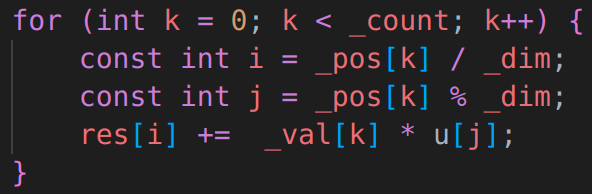
\includegraphics[width=0.8\linewidth]{matrix_vector_man2.png}
    \end{center}
\end{itemize}

        
        \column{.3\textwidth} % Right column and width
        $ \left( \begin{array}{rrrrr} 
0 & 5.3 & 0 & 0 & 1.5\\ 
4.2 & 0& 3.1 & 0 & 2\\ 
0 & 0 & 0 & 0 & 0 \\
0 & 0 & 0 & 2.2 & 0 \\
1.9 & 0 & 0 & 0 & 0
\end{array} \right) $

    \end{columns}
\end{frame}

%------------------------------------------------

\begin{frame}{Matrix-Vector multiplication: Sparse - CSR}
    \begin{columns}[c] % The "c" option specifies centered vertical alignment while the "t" option is used for top vertical alignment

\column{.65\textwidth} % Left column and width
\begin{itemize}
\item sparse - csr (compressed row storage)
	\begin{itemize}
       \item $\mathrm{values} = \begin{bmatrix}
		5.3, & 1.5, & 4.2, & 3.1, & 2, & 2.2, & 1.9 
		\end{bmatrix}$
		\item $\mathrm{col\_ind} = \begin{bmatrix}
		1, & 4, & 0, & 2, & 4, & 3, & 0 
		\end{bmatrix}$
		\item $\mathrm{row\_ptr} = \begin{bmatrix}
		0, & 2, & 5, & 5, & 6, & 7 
		\end{bmatrix}$
	\end{itemize}
\item matrix-vector multiplication
\begin{center}
    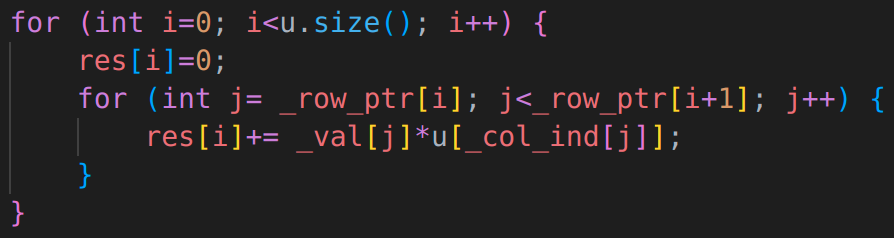
\includegraphics[width=0.8\linewidth]{matrix_vector_csr.png}
    \end{center}
\end{itemize}
        
        \column{.3\textwidth} % Right column and width
        $ \left( \begin{array}{rrrrr} 
0 & 5.3 & 0 & 0 & 1.5\\ 
4.2 & 0& 3.1 & 0 & 2\\ 
0 & 0 & 0 & 0 & 0 \\
0 & 0 & 0 & 2.2 & 0 \\
1.9 & 0 & 0 & 0 & 0
\end{array} \right) $

    \end{columns}
\end{frame}

%------------------------------------------------
\begin{frame}{Solution: Sparse but not scarce}
    \begin{itemize}
        \item two self-implemented classes for sparse matrices: non-CSR and CSR format.
        \item Eigen library
        \begin{itemize}
        	\item added to repository as a git submodule
        	\item SparseMatrix class
        	\item SparseMatrix::makeCompressed() conversion to CSR format
        	\item forward Euler simplified using matrix multiplication notation: 	
        \end{itemize}
    \end{itemize}	
    \centerline{Eigen::SparseMatrix B * Eigen::VectorXd u}
\end{frame}

%------------------------------------------------


\begin{frame}{Google Benchmark}
    \begin{itemize}
        \item github.com/google/benchmark
        \item a library to benchmark code snippets (functions) 
        \item added to repository as a git submodule
    \end{itemize}
    
    \begin{center}
    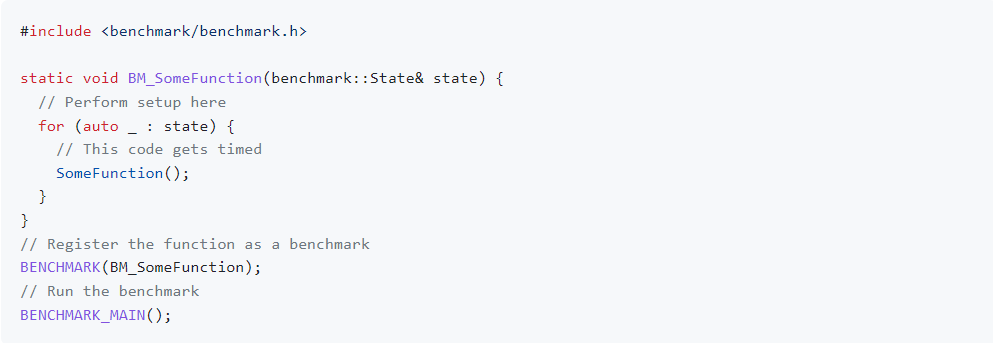
\includegraphics[width=0.8\linewidth]{example_google_benchmark.png}
    \end{center}
\end{frame}

%------------------------------------------------

\begin{frame}{Code organization}
    \begin{itemize}
        \item Cmake build 8 targets, common + unique code
        \item 4 versions of PDE solver
        \item corresponding benchmarks, testing functions unique to each implementation 
    \end{itemize}
    
    \begin{center}
    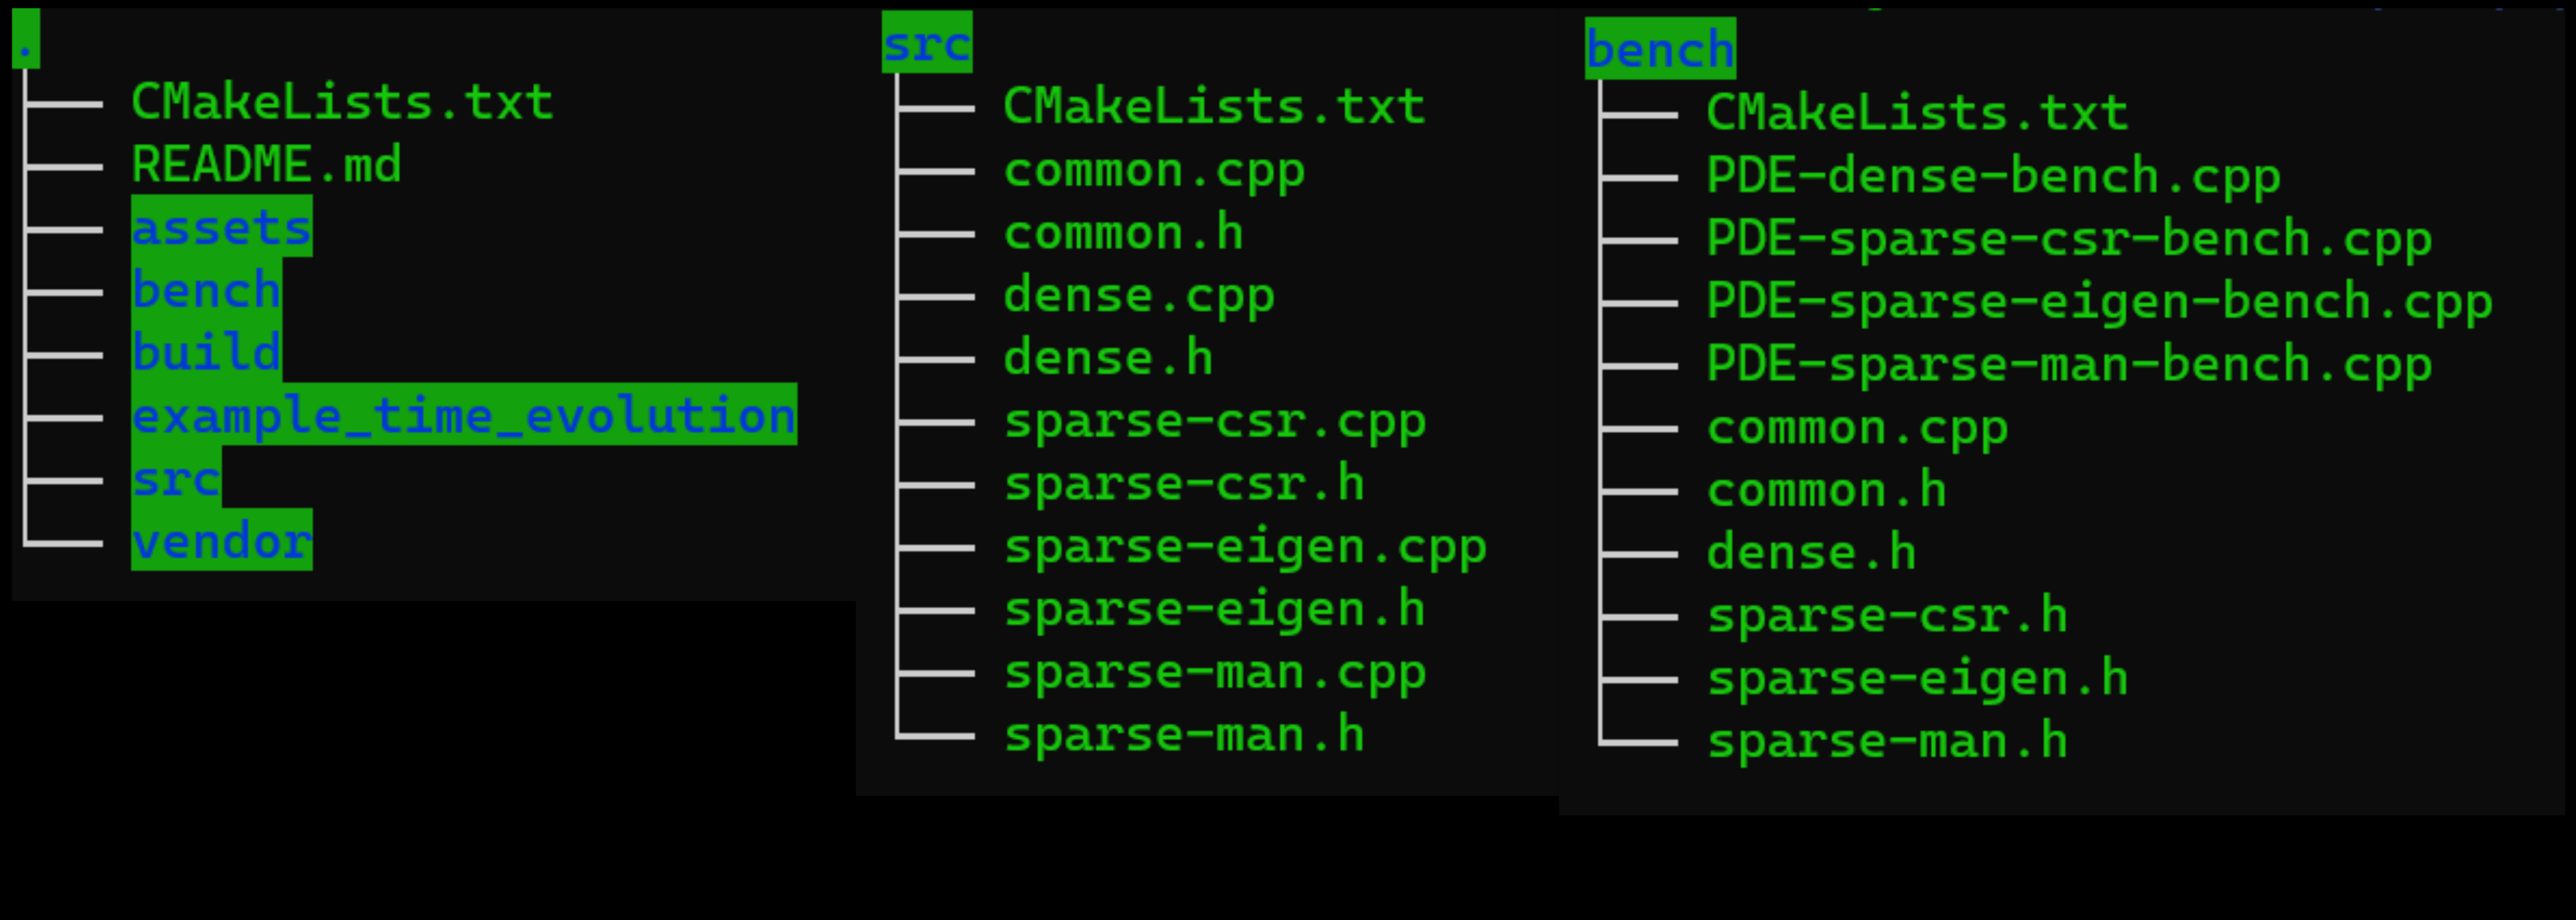
\includegraphics[width=0.8\linewidth]{code_structure.png}
    \end{center}
\end{frame}

%------------------------------------------------

\begin{frame}{Benchmark example output}
   \begin{center}
   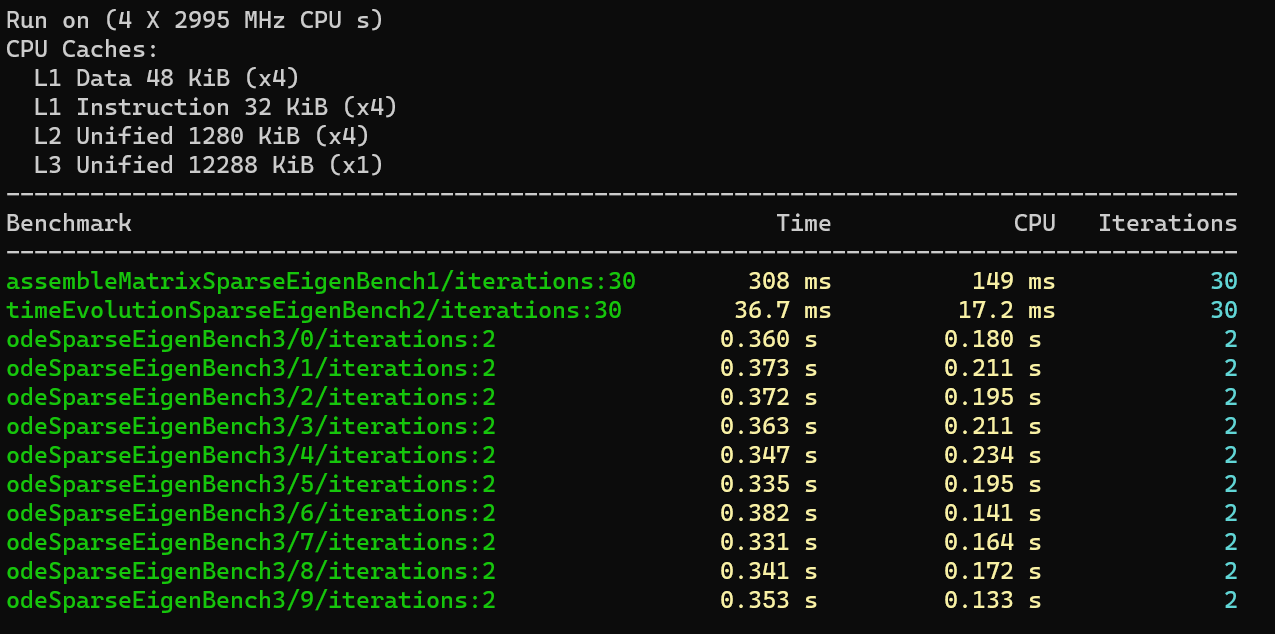
\includegraphics[width=0.8\linewidth]{example_benchmark.png}
   \end{center}
\end{frame}

%------------------------------------------------

\begin{frame}{Benchmark assembly matrix B}
   
    \begin{itemize}
        \item 30 iterations
        \item Linux (Martin's machine), Windows and WSL (Charlotte's machine)
    \end{itemize}
    
    \begin{center}
   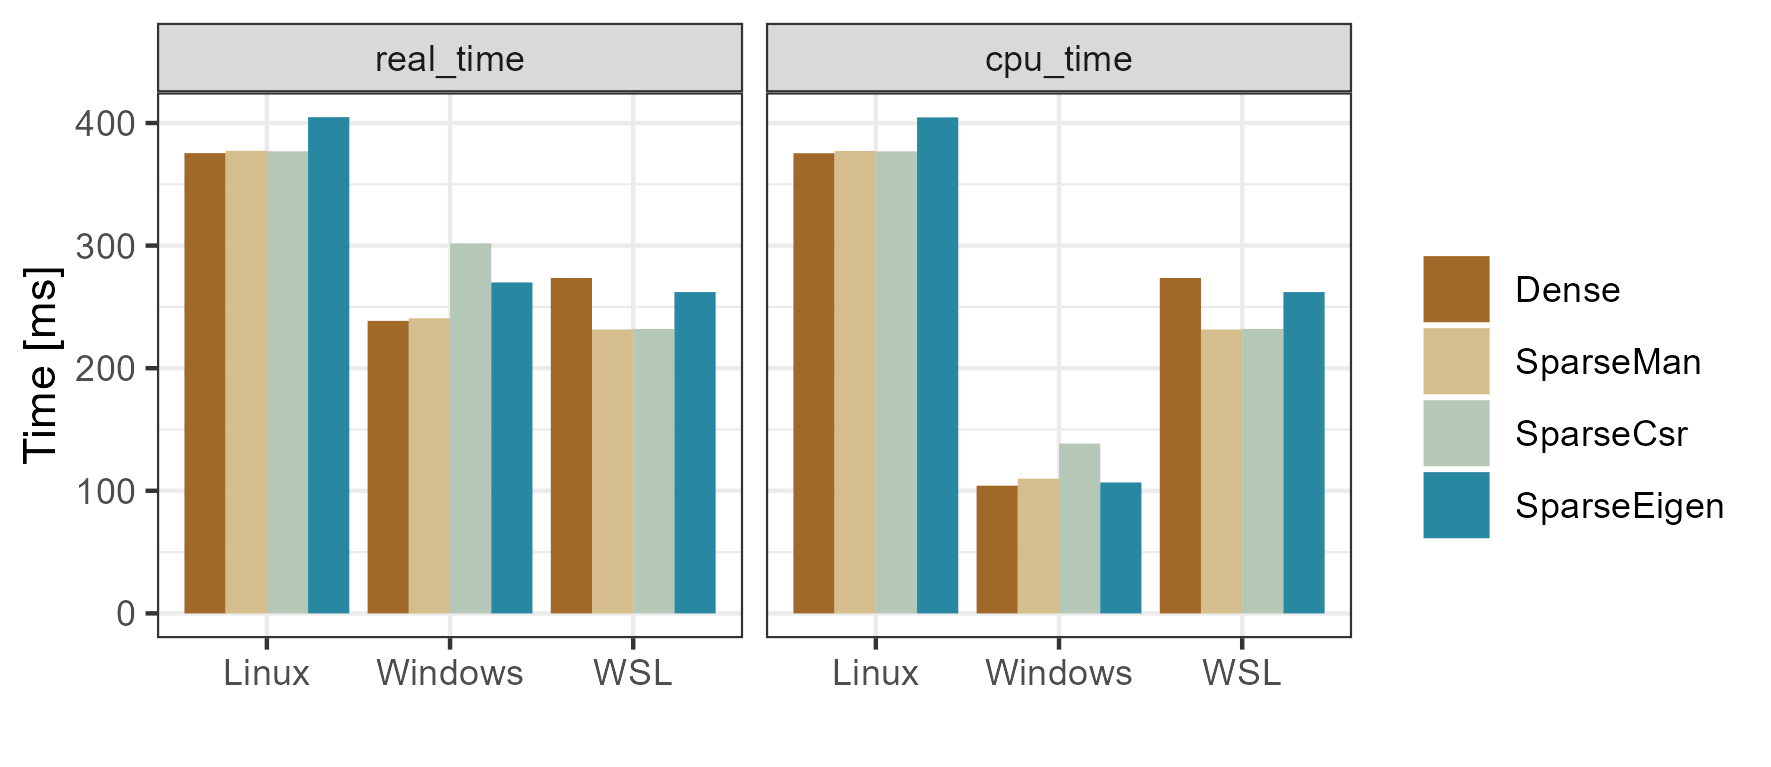
\includegraphics[width=0.8\linewidth]{assembly_bench_result.png}
   \end{center}
   
\end{frame}

%------------------------------------------------

\begin{frame}{Benchmark time evolution}
   
    \begin{itemize}
        \item 30 iterations
    \end{itemize}
    
    \begin{center}
   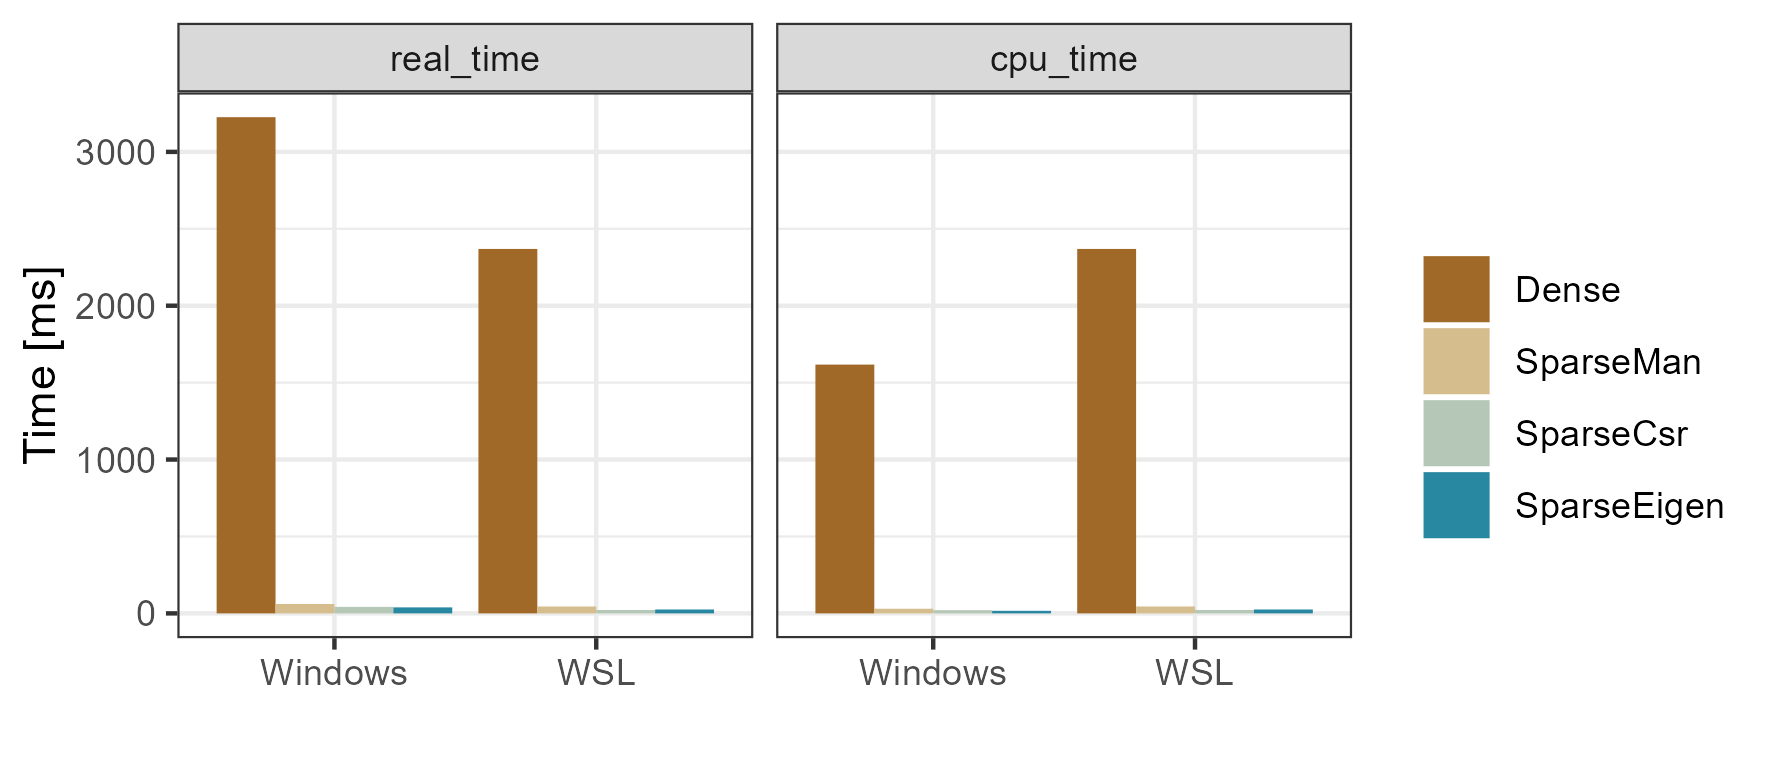
\includegraphics[width=0.8\linewidth]{timeevolution_bench_result.png}
   \end{center}
   
\end{frame}

%------------------------------------------------

\begin{frame}{Benchmark time evolution}
   
    \begin{itemize}
        \item 30 iterations
    \end{itemize}
    
    \begin{center}
   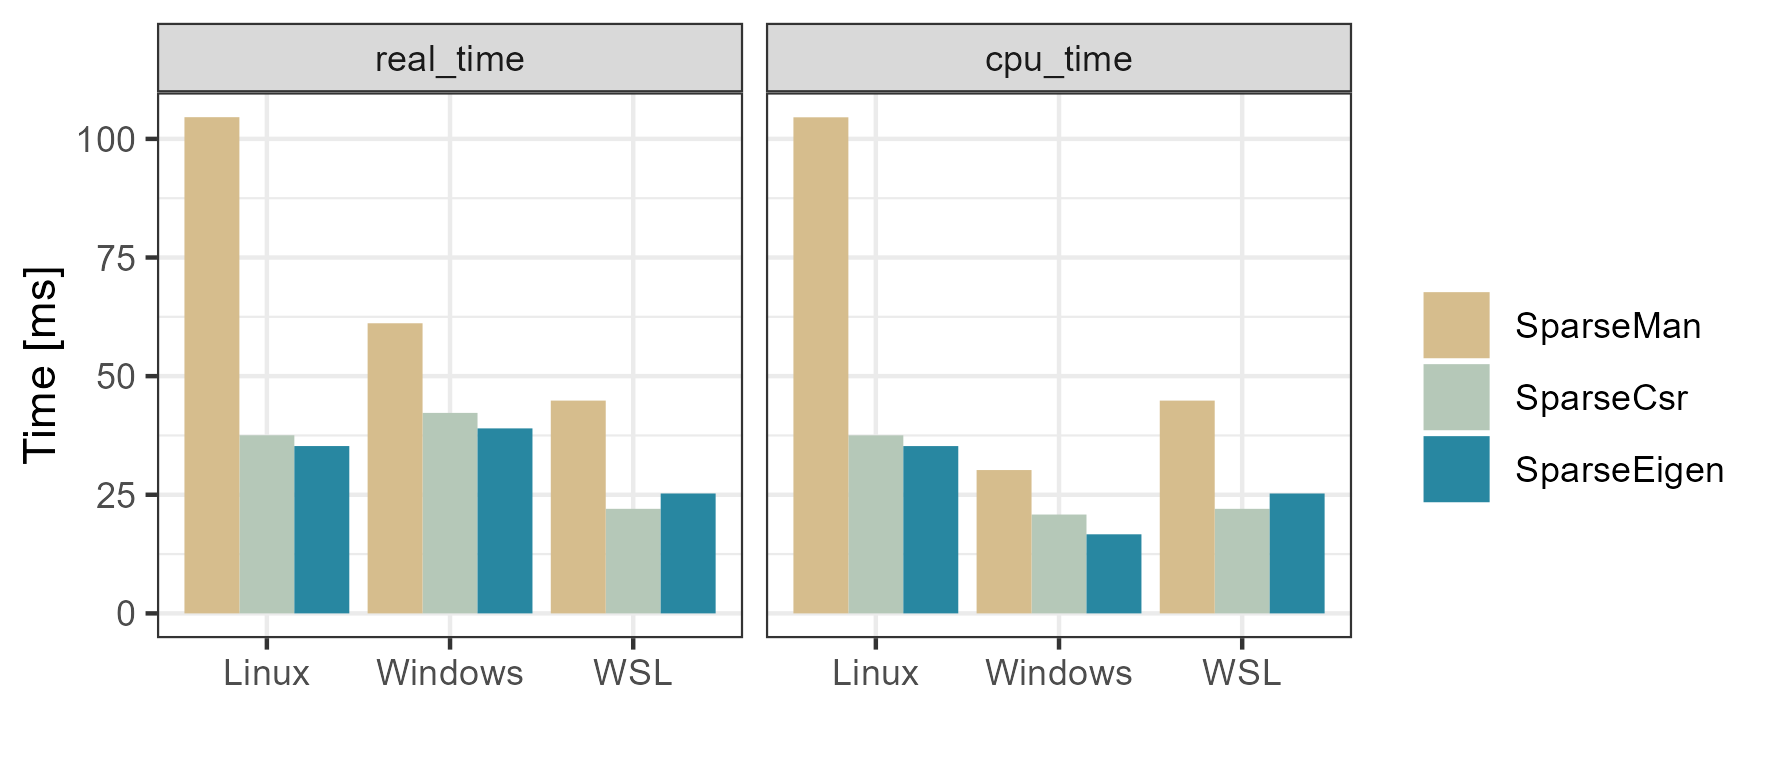
\includegraphics[width=0.8\linewidth]{timeevolution_bench_result2.png}
   \end{center}
   
\end{frame}

%------------------------------------------------

\begin{frame}{Benchmark time evolution}
   
    \begin{itemize}
        \item 2 iterations, for different timesteps (dt)
    \end{itemize}
    
    \begin{center}
   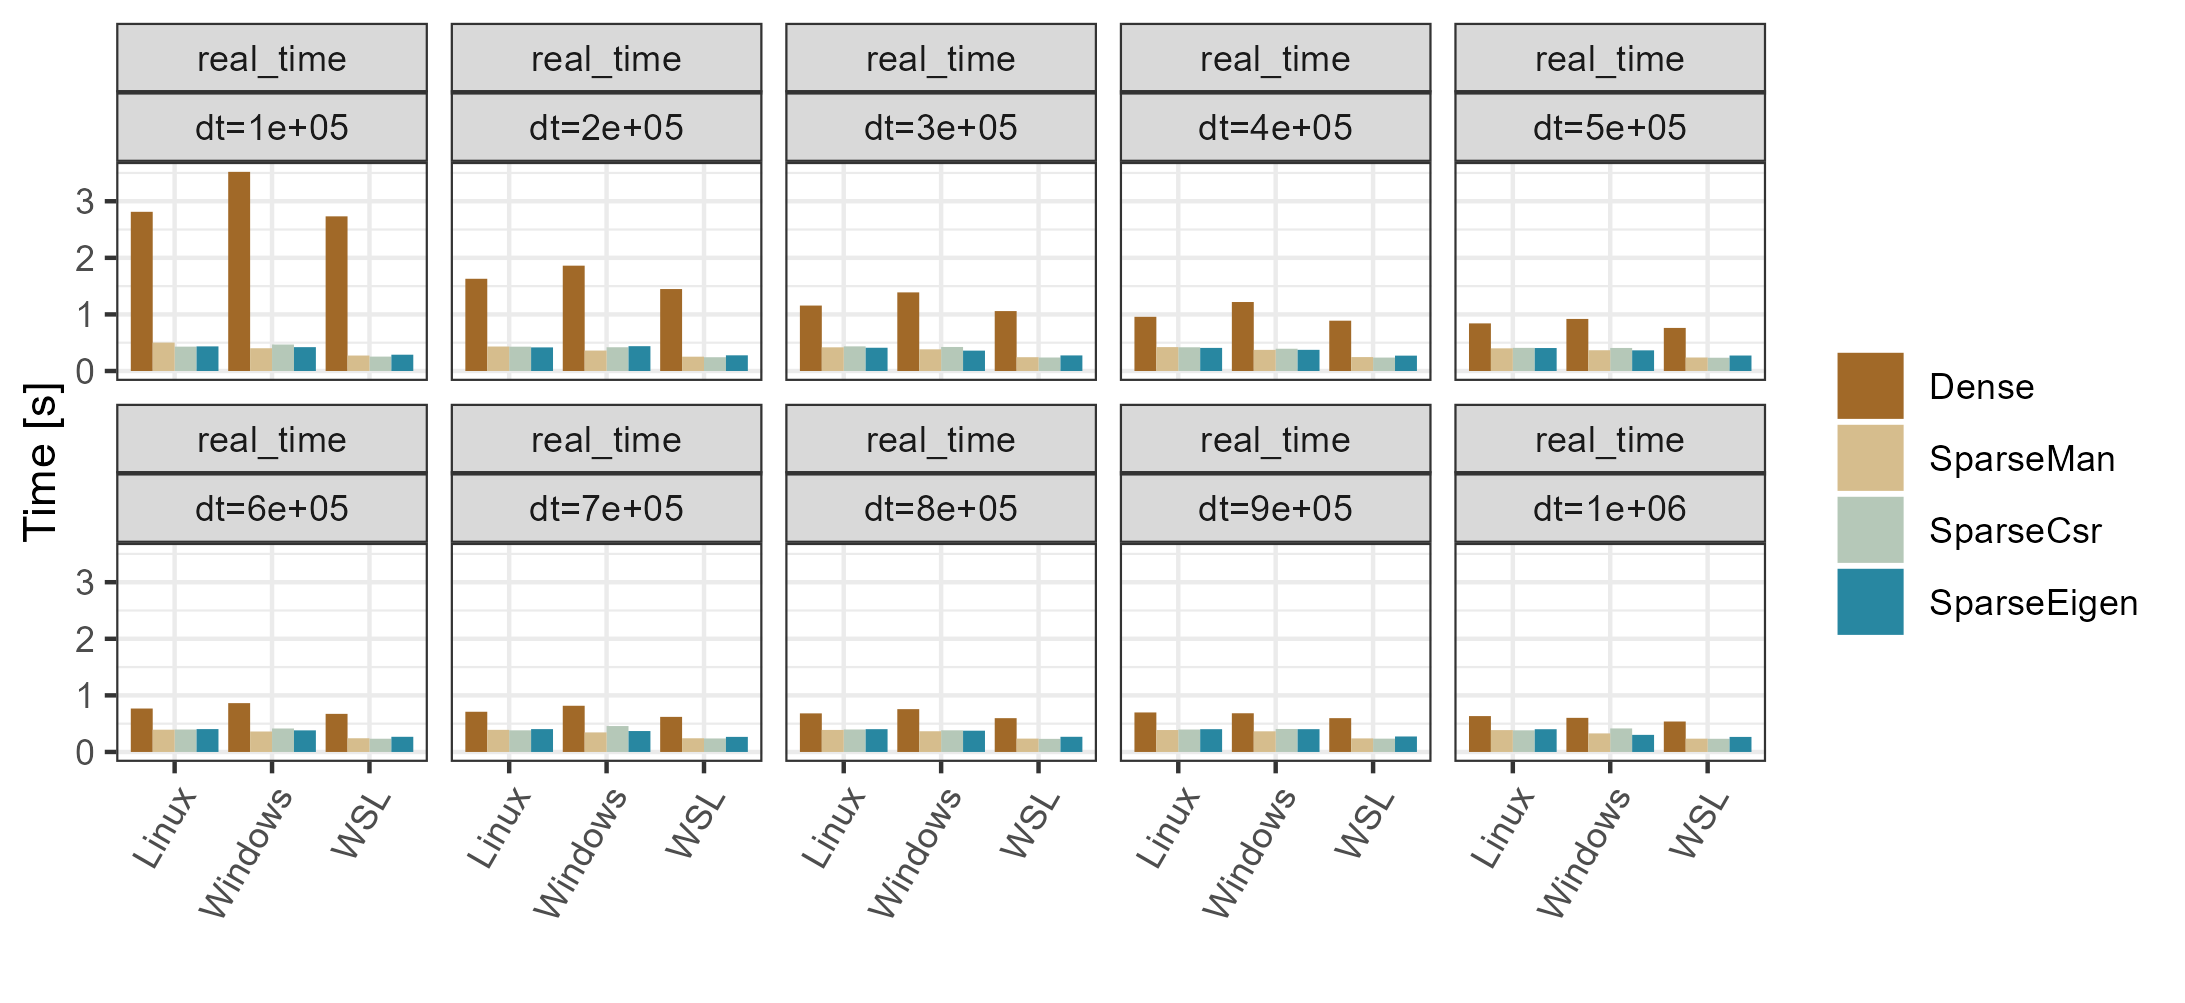
\includegraphics[width=1\linewidth]{ode_bench_result.png}
   \end{center}
   
\end{frame}

%------------------------------------------------

\begin{frame}{Conclusions}
   \begin{itemize}
      \item Sparse formats preferred over dense format:
   	 \begin{itemize}
   	  \item Memory issues for large mesh sizes
	  \item Time needed for matrix assembly similar (dependence on machine and OS used?)
	  \item Significant 100-fold time-speed up using sparse format for time evolution
     \end{itemize}
   	 \item Tradeoff own sparse format vs CSR-format:
   	 \begin{itemize}
	  \item Extra time needed for converting COO to CSR 
	  \item Speed up at time evolution
	  
	  \end{itemize}
	  \item Tradeoff library vs own implementation:
	  \begin{itemize}
	  \item Time spent on learning the library (once) vs on correctly implementing the sparse format
	  \item With Eigen code simplification using matrix product expressions
	  \end{itemize}
   \end{itemize}
\end{frame}

%------------------------------------------------

\begin{frame}
    \Huge{\centerline{Questions?}}
\end{frame}

\end{document}